\documentclass[type=wiki,gwikiid=functor]{gwiki}

%% ============================================================================
%% Functor
%% GWiki Note - Definition
%% ============================================================================

\GWikiMeta{functor}{Functor}{wiki}[category-theory, definition]
\GWikiDate{2025-12-08}
\GWikiSummary{%
  A functor is a structure-preserving map between categories, mapping objects
  to objects and morphisms to morphisms while respecting composition and identities.
}

\begin{document}

\gwikinoteheader

%% ============================================================================
%% Definition
%% ============================================================================

\begin{definition}[Functor]
  Let $\cC$ and $\cD$ be \wref{category}[categories]. A \concept{functor}
  $F : \cC \to \cD$ consists of:
  \begin{lst}
    \item An \term{object function}: for each $A \in \Obj(\cC)$, an object
          $F(A) \in \Obj(\cD)$
    \item A \term{morphism function}: for each $f : A \to B$ in $\cC$, a morphism
          $F(f) : F(A) \to F(B)$ in $\cD$
  \end{lst}
  satisfying the \term{functoriality axioms}:
  \begin{lst}
    \item $F(\id_A) = \id_{F(A)}$ for all objects $A$
    \item $F(g \circ f) = F(g) \circ F(f)$ for all composable morphisms
  \end{lst}
\end{definition}

%% ============================================================================
%% Variants
%% ============================================================================

\begin{definition}[Contravariant functor]
  A \concept{contravariant functor} $F : \cC \to \cD$ is a functor
  $F : \cC^\op \to \cD$. Equivalently, it reverses the direction of morphisms:
  $f : A \to B$ maps to $F(f) : F(B) \to F(A)$.
\end{definition}

\begin{remark}
  When we say ``functor'' without qualification, we mean a \term{covariant functor}.
\end{remark}

%% ============================================================================
%% Examples
%% ============================================================================

\begin{example}[Forgetful functors]
  The \term{forgetful functor} $U : \Grp \to \Set$ sends each group to its
  underlying set and each homomorphism to its underlying function.
\end{example}

\begin{example}[Free functors]
  The \term{free functor} $F : \Set \to \Grp$ sends each set $X$ to the
  free group $F(X)$ generated by $X$.
\end{example}

\begin{example}[Hom functors]
  For any object $A$ in a locally small category $\cC$:
  \begin{lst}
    \item $\Hom(A, -) : \cC \to \Set$ is a covariant functor
    \item $\Hom(-, A) : \cC^\op \to \Set$ is a contravariant functor
  \end{lst}
\end{example}

\begin{example}[Power set functor]
  The power set functor $\cP : \Set \to \Set$ sends $X$ to $\cP(X)$ and
  $f : X \to Y$ to the direct image $f_* : \cP(X) \to \cP(Y)$.
\end{example}

%% ============================================================================
%% Properties
%% ============================================================================

\begin{proposition}
  Functors compose: if $F : \cC \to \cD$ and $G : \cD \to \cE$ are functors,
  then $G \circ F : \cC \to \cE$ is a functor.
\end{proposition}

\begin{definition}[Functor category]
  Given categories $\cC$ and $\cD$, the \concept{functor category} $[\cC, \cD]$
  or $\cD^\cC$ has:
  \begin{lst}
    \item Objects: functors $F : \cC \to \cD$
    \item Morphisms: \wref{natural-transformation}[natural transformations]
  \end{lst}
\end{definition}

%% ============================================================================
%% Diagram
%% ============================================================================

A functor preserves the ``shape'' of diagrams:

\begin{center}
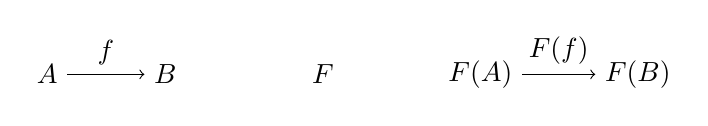
\begin{tikzpicture}[node distance=1.5cm]
  % Source category
  \node (A) {$A$};
  \node (B) [right of=A] {$B$};
  \draw[->] (A) -- node[above] {$f$} (B);

  % Arrow for functor
  \node (F) [right of=B, xshift=0.5cm] {$\xmapsto{F}$};

  % Target category
  \node (FA) [right of=F, xshift=0.5cm] {$F(A)$};
  \node (FB) [right of=FA, xshift=0.5cm] {$F(B)$};
  \draw[->] (FA) -- node[above] {$F(f)$} (FB);
\end{tikzpicture}
\end{center}

%% ============================================================================
%% Related Concepts
%% ============================================================================

\seealso{category, natural-transformation, adjunction, yoneda-lemma}

\gwikifooter

\end{document}
